\chapter{Discussion}

None of the approaches compared in the preceding chapter is flawless, and each works better under certain circumstances. Our implementation gives the user an option to choose the approach and experiment with the results. \Cref{fig:composed_drawings} shows that in many cases, the results are similar across different selected approaches. The random nature of the Monte Carlo algorithm allows generating multiple different drawings for one description. This randomness increases the chances that the generated image will eventually correspond with the input description. Future research might focus on automatic scoring and cherry-picking of the generated scenes. Other possible improvements may be achieved by employing more advanced machine-learning models used for constraints and size prediction. Our implementation relies on a simple rule-based description processing which is sufficient for simple sentences; However, finding a better approach may also be a subject of future research.

\begin{figure}[ht]
    \captionsetup[subfigure]{labelformat=empty}
    \centering
        \begin{subfigure}{\textwidth}
            \centering
            \caption{(1) \say{A dog and a cat are sitting on a couch. The couch is in a house and there is a tree next to the house.}}
            \begin{subfigure}[t]{0.45\textwidth}
                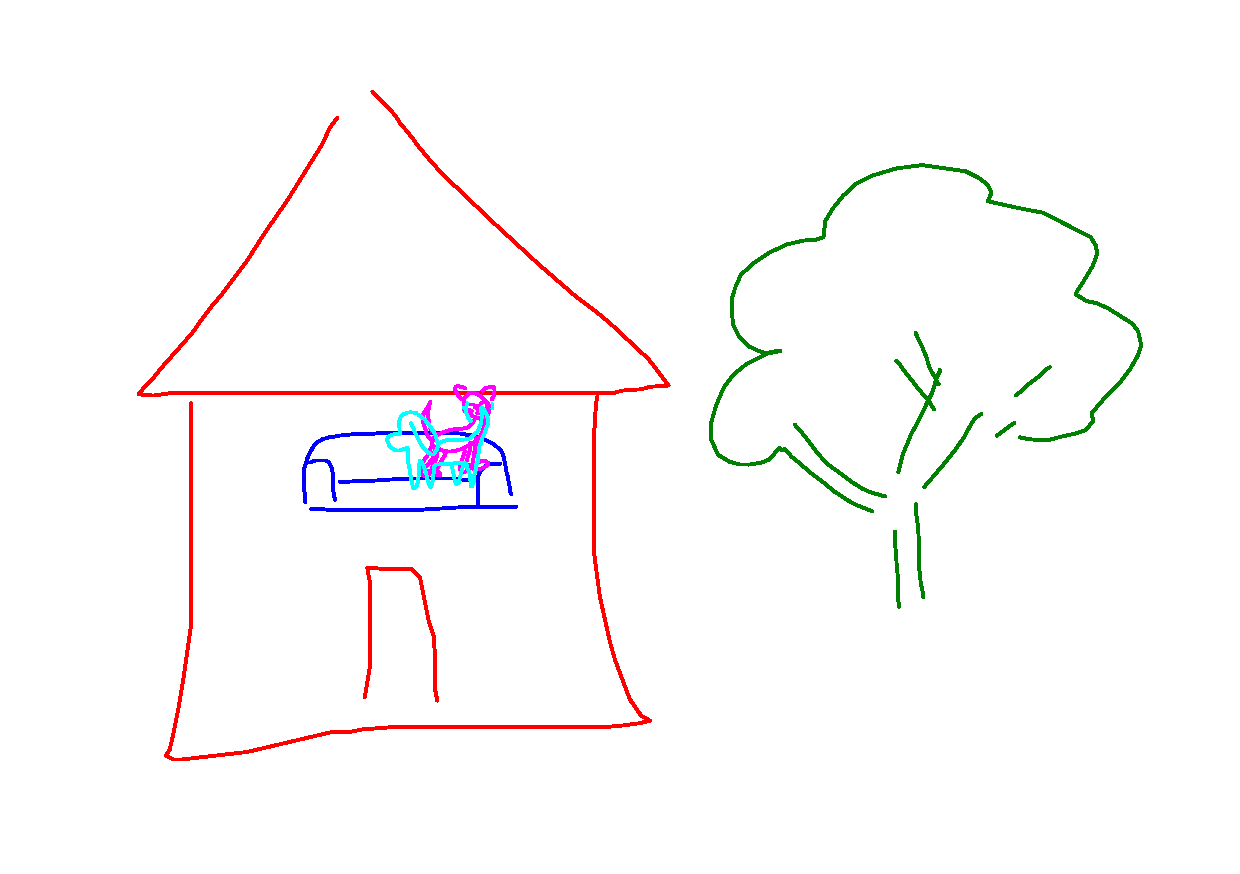
\includegraphics[width=\textwidth]{figures/drawing_1_ra.pdf}
                \caption{rule-based constraints, absolute sizes}
            \end{subfigure}
            \hfill
            \begin{subfigure}[t]{0.45\textwidth}
                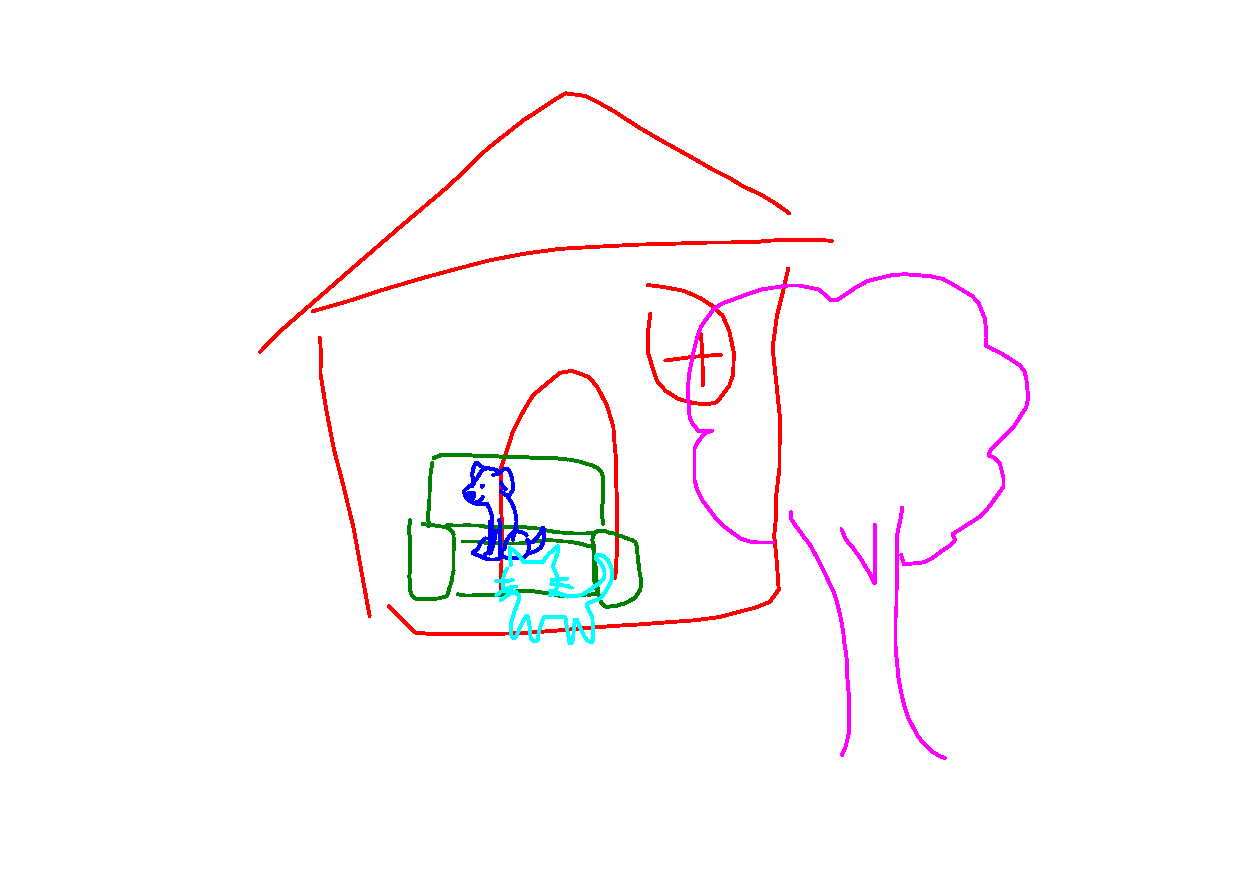
\includegraphics[width=\textwidth]{figures/drawing_1_ca.pdf}
                \caption{classifier-based constraints, absolute sizes}
            \end{subfigure}
        \end{subfigure}
        \begin{subfigure}{\textwidth}
            \centering
            \caption{(2) \say{Two ducks are swimming in a pond which is next to a tree. a bench is under the tree.}}
            \begin{subfigure}{0.45\textwidth}
                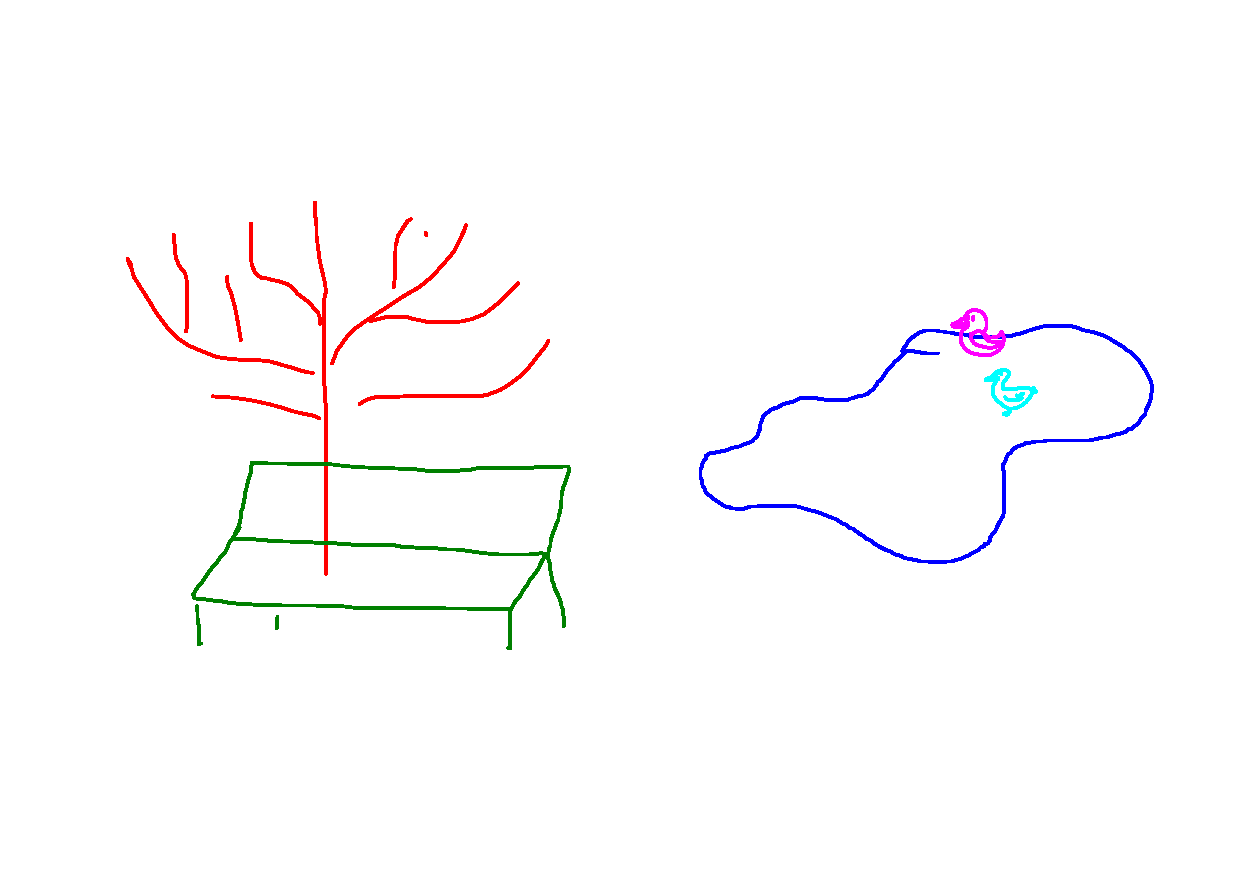
\includegraphics[width=\textwidth]{figures/drawing_2_ca.pdf}
                \caption{classifier-based constraints, absolute sizes}
            \end{subfigure} 
            \hfill
            \begin{subfigure}{0.45\textwidth}
                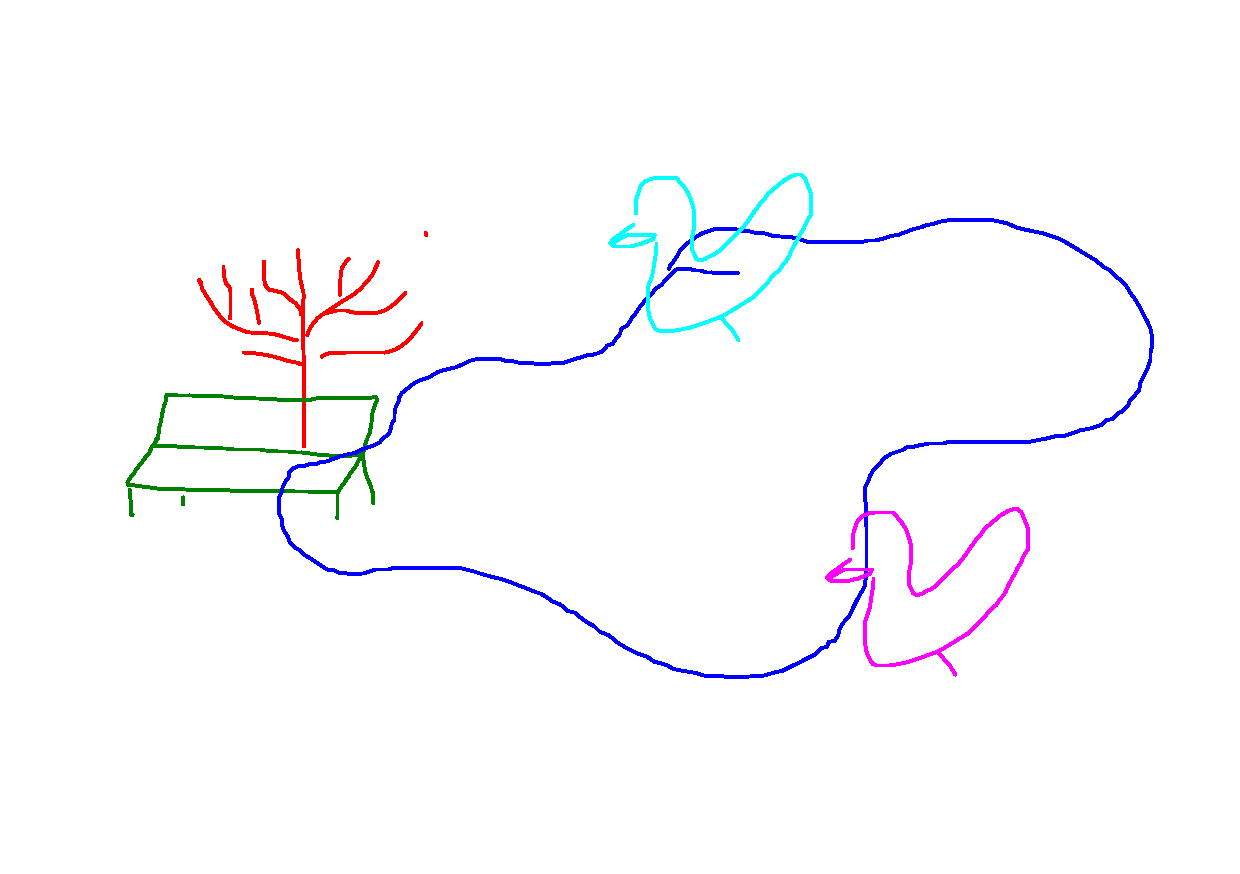
\includegraphics[width=\textwidth]{figures/drawing_2_cr.pdf}
                \caption{classifier-based constraints, relative sizes}
            \end{subfigure}
        \end{subfigure}
        \begin{subfigure}{\textwidth}
            \centering
            \caption{(3) \say{There is a house, and mountains behind it. The sun is rising above the mountains.}}
            \begin{subfigure}[t]{0.45\textwidth}
                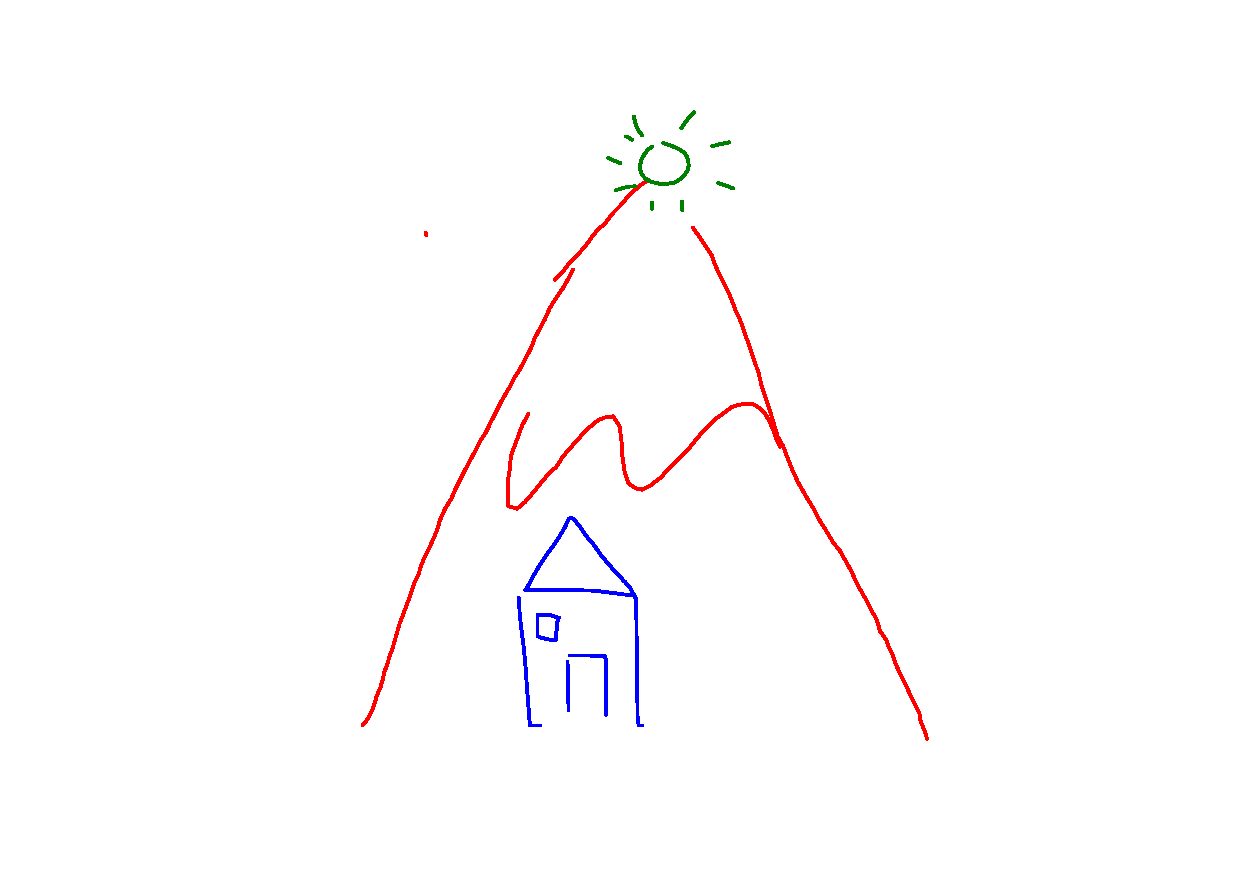
\includegraphics[width=\textwidth]{figures/drawing_3_rr.pdf} 
                \caption{rule-based constraints, relative sizes}
            \end{subfigure}
            \hfill
            \begin{subfigure}[t]{0.45\textwidth}
                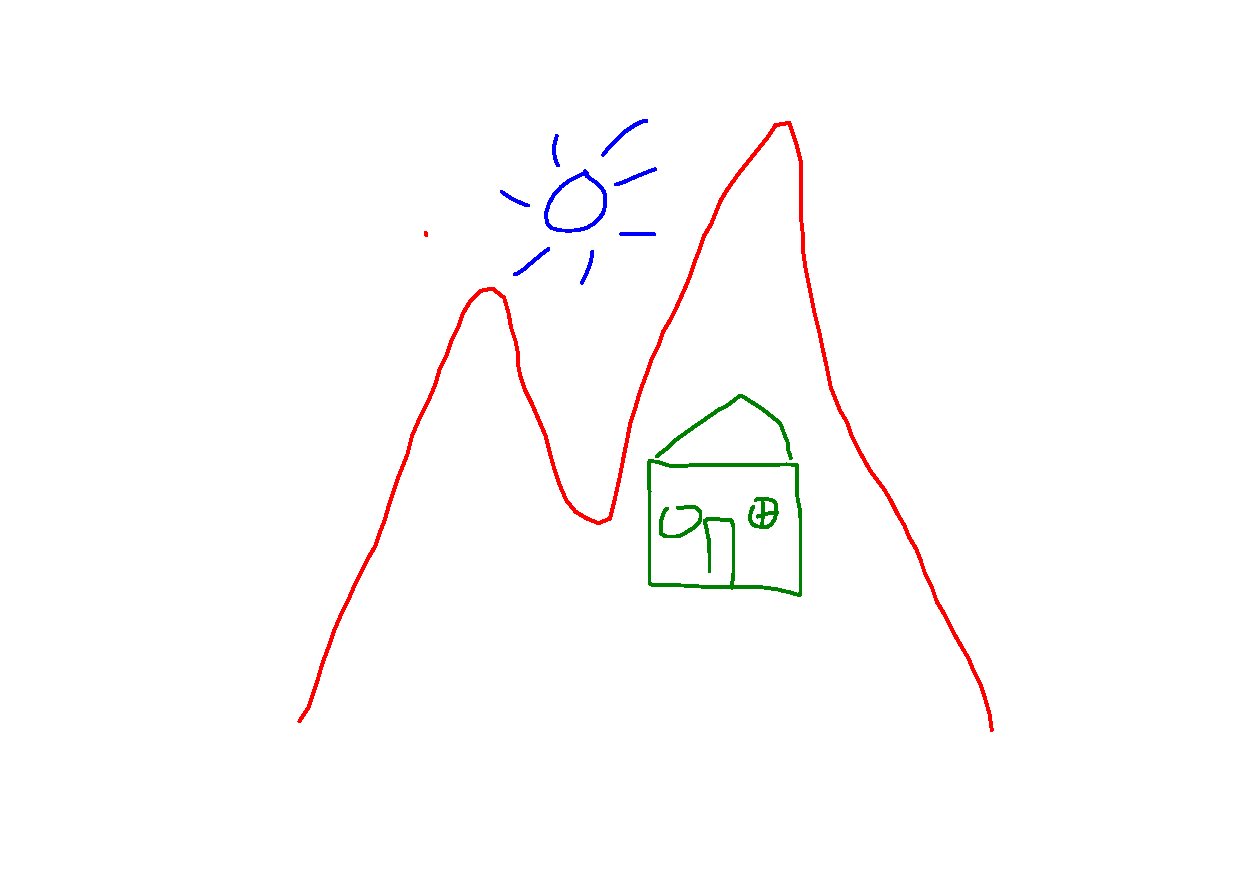
\includegraphics[width=\textwidth]{figures/drawing_3_cr.pdf}
                \caption{classifier-based constraints, relative sizes}
            \end{subfigure}
        \end{subfigure}
    \caption[Examples of generated drawings]{Examples of generated drawings. Each example is labelled with the used approach for determining the position and size. The absolute sizes refer to the hand crafted absolute size table.}
    \label{fig:composed_drawings}
\end{figure}
